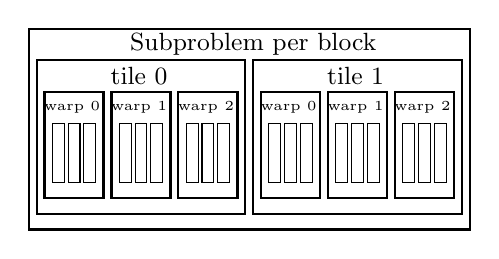
\begin{tikzpicture}[every node/.style={thick,rectangle,inner sep=0pt}]
\def \dx {0.05}
\def \dy {0.2}
\def \recx {0.15}
\def \recX {3*\recx + 4*\dx}
\def \recXX {3 * \recX + 22 * \dx}
\def \recy {0.75}
\def \recY {\recy + 3 * \dy}
\def \recYY {\recY + 3 * \dy}

%% left child 
\draw [black] (0 + 0, 0 + 0) rectangle (0 + \recx, 0 + \recy);
\draw [black] (0 + \recx + \dx, 0) rectangle (0 + 2*\recx + \dx, 0 + \recy);
\draw [black] (0 + 2*\recx + 2*\dx, 0 + 0) rectangle (0 + 3*\recx + 2*\dx, 0 + \recy);

\draw[thick, black] (0-2*\dx, 0-\dy) rectangle (0-2*\dx + \recX + 2 * \dx, 0-\dy + \recY);
\node () at (0 + 1 * \recx + 2 * \dx, \recy + \dy) {\tiny warp 0};

\draw [black] (\recX + 4*\dx + 0, 0 + 0) rectangle (\recX + 4*\dx + \recx, 0 + \recy);
\draw [black] (\recX + 4*\dx + \recx + \dx, 0) rectangle (\recX + 4*\dx + 2*\recx + \dx, 0 + \recy);
\draw [black] (\recX + 4*\dx + 2*\recx + 2*\dx, 0 + 0) rectangle (\recX + 4*\dx + 3*\recx + 2*\dx, 0 + \recy);

\draw[thick, black] (\recX + 4*\dx-2*\dx, 0-\dy) rectangle (\recX + 4*\dx-2*\dx + \recX + 2 * \dx, 0-\dy + \recY);
\node () at (\recX + 4*\dx + 1 * \recx + 2 * \dx, \recy + \dy) {\tiny warp 1};

\draw [black] (2*\recX + 12*\dx + 0, 0 + 0) rectangle (2*\recX + 12*\dx + \recx, 0 + \recy);
\draw [black] (2*\recX + 12*\dx + \recx + \dx, 0) rectangle (2*\recX + 12*\dx + 2*\recx + \dx, 0 + \recy);
\draw [black] (2*\recX + 12*\dx + 2*\recx + 2*\dx, 0 + 0) rectangle (2*\recX + 12*\dx + 3*\recx + 2*\dx, 0 + \recy);

\draw[thick, black] (2*\recX + 12*\dx-2*\dx, 0-\dy) rectangle (2*\recX + 12*\dx-2*\dx + \recX + 2 * \dx, 0-\dy + \recY);
\node () at (2*\recX + 12*\dx + 1 * \recx + 2 * \dx, \recy + \dy) {\tiny warp 2};

\draw [thick, black] (0-4*\dx, 0-2*\dy) rectangle (0-4*\dx + \recXX, 0-2*\dy + \recYY);
\node () at (\recX + 4*\dx + 1 * \recx + 2 * \dx, \recy + 3* \dy) {\small tile 0};

%% right child
\draw [black] (\recXX + 2*\dx + 0, 0 + 0) rectangle (\recXX +2*\dx+ \recx, 0 + \recy);
\draw [black] (\recXX + 2*\dx + \recx + \dx, 0) rectangle (\recXX +2*\dx+ 2*\recx + \dx, 0 + \recy);
\draw [black] (\recXX + 2*\dx + 2*\recx + 2*\dx, 0 + 0) rectangle (\recXX +2*\dx+ 3*\recx + 2*\dx, 0 + \recy);

\draw[thick, black] (\recXX, 0-\dy) rectangle (\recXX + \recX + 2 * \dx, 0-\dy + \recY);
\node () at (\recXX + 2*\dx +  1 * \recx + 2 * \dx, \recy + \dy) {\tiny warp 0};

\draw [black] (\recXX + 2*\dx+\recX + 4*\dx + 0, 0 + 0) rectangle (\recXX + 2*\dx+\recX + 4*\dx + \recx, 0 + \recy);
\draw [black] (\recXX + 2*\dx+\recX + 4*\dx + \recx + \dx, 0) rectangle (\recXX + 2*\dx+\recX + 4*\dx + 2*\recx + \dx, 0 + \recy);
\draw [black] (\recXX + 2*\dx+\recX + 4*\dx + 2*\recx + 2*\dx, 0 + 0) rectangle (\recXX + 2*\dx+\recX + 4*\dx + 3*\recx + 2*\dx, 0 + \recy);

\draw[thick, black] (\recXX + 2*\dx+\recX + 4*\dx-2*\dx, 0-\dy) rectangle (\recXX + 2*\dx+\recX + 4*\dx-2*\dx + \recX + 2 * \dx, 0-\dy + \recY);
\node () at (\recXX + 2*\dx+\recX + 4*\dx + 1 * \recx + 2 * \dx, \recy + \dy) {\tiny warp 1};

\draw [black] (\recXX + 2*\dx + 2*\recX + 12*\dx + 0, 0 + 0) rectangle (\recXX + 2*\dx + 2*\recX + 12*\dx + \recx, 0 + \recy);
\draw [black] (\recXX + 2*\dx + 2*\recX + 12*\dx + \recx + \dx, 0) rectangle (\recXX + 2*\dx + 2*\recX + 12*\dx + 2*\recx + \dx, 0 + \recy);
\draw [black] (\recXX + 2*\dx + 2*\recX + 12*\dx + 2*\recx + 2*\dx, 0 + 0) rectangle (\recXX + 2*\dx + 2*\recX + 12*\dx + 3*\recx + 2*\dx, 0 + \recy);

\draw[thick, black] (\recXX + 2*\dx + 2*\recX + 12*\dx-2*\dx, 0-\dy) rectangle (\recXX + 2*\dx + 2*\recX + 12*\dx-2*\dx + \recX + 2 * \dx, 0-\dy + \recY);
\node () at (\recXX + 2*\dx + 2*\recX + 12*\dx + 1 * \recx + 2 * \dx, \recy + \dy) {\tiny warp 2};

\draw [thick, black] (\recXX-2*\dx, 0-2*\dy) rectangle (\recXX-2*\dx + \recXX, 0-2*\dy + \recYY);
\node () at (\recXX  + 2*\dx + \recX + 4*\dx + 1 * \recx + 2 * \dx, \recy + 3* \dy) {\small tile 1};

%% subproblem per block:
\draw [thick, black] (0-6*\dx, 0 - 3 * \dy) rectangle (0-6*\dx + 3*\recXX + 5*\dx, 0-3*\dy + \recYY + 3*\dy);
\node () at (\recXX -2* \dx, \recYY -\dy) {\small Subproblem per block};
\end{tikzpicture}